%!TeX TXS-program:bibliography = txs:///biber
\documentclass{article}

% other stuff
\usepackage[dvipsnames]{xcolor}
\usepackage{fullpage}
\usepackage{graphicx}
\usepackage{authblk}
\usepackage{booktabs}
\usepackage[%
plainpages=false,%
colorlinks,% removes the boxes around links
urlcolor=black,%
filecolor=black,%
citecolor=Blue,%   requires xcolor with option dvipsnames
linkcolor=black,%
pdfpagemode=UseOutlines,%
pdfauthor={Lars Vilhuber},%
pdfsubject={Economics, Reproducibility, Open Science},%
]{hyperref}

\usepackage[
backend=biber,
authordate,
  noibid,
  natbib,
  sorting=nyt,
  sortcites=true
  abbreviate=false,
  citetracker=false,
  isbn=false,ibidtracker=false]{biblatex-chicago}

\defbibfilter{papers}{
     type=article or
     type=inproceedings or
     type=conference or
     type=proceedings or
     type=incollection or
     type=inbook
}
% Clear some stuff from the bibliography
\AtEveryBibitem{%
        \clearfield{day}%
        \clearfield{month}%
        \clearfield{endday}%
        \clearfield{endmonth}%
    \clearlist{language}%
    \clearfield{issn}%
    \clearfield{eprint}% - adjust if necessary
    \iffieldundef{doi}{}{\clearfield{url}}% remove URL field if DOI present    
}

% acronyms
\usepackage{acronym}

\acrodef{AEA}{American Economic Association}
\acrodef{AI}{artificial intelligence}
\acrodef{AJPS}{American Journal of Political Science}
\acrodef{BPLIM}{Banco de Portugal Microdata Research Laboratory}
\acrodef{BLS}{Bureau of Labor Statistics}
\acrodef{CASD}{Centre d'accès sécurisé aux données}
\acrodef{CC-BY}{Creative Commons Attribution}
\acrodef{CIQSS}{Centre interuniversitaire québécois de statistiques sociales}
\acrodef{CEA}{Canadian Economics Association}
\acrodef{CJE}{Canadian Journal of Economics}
\acrodef{CSWEP}{AEA Committee on the Status of Women in the Economics Profession}
\acrodef{DCAP}{data and code availability policy}
\acrodef{DCAS}{Data and Code Availability Standard}
\acrodef{DHS}{Demographic and Health Surveys}
\acrodef{DOI}{Digital Object Identifier}
\acrodef{EEA}{European Economics Association}
\acrodef{EJ}{Economic Journal}
\acrodef{EI}{Economic Inquiry}
\acrodef{ERS}{Economic Research Service}
\acrodef{FAIR}{Findable, Accessible, Interoperable, Re-usable}
\acrodef{FAQ}{frequently asked questions}
\acrodef{FSRDC}{Federal Statistical Research Data Centers}
\acrodef{GDPR}{General Data Protection Regulation}
\acrodef{GIS}{geographical information system}
\acrodef{GPU}{graphical processing unit}
\acrodef{HRS}{Health and Retirement Study}
\acrodef{IAB}{Research Data Center (FDZ) at the Institute for Employment Research}
\acrodef{IRS}{Internal Revenue Service}
\acrodef{IRB}{institutional review board}
\acrodef{ICPSR}{Inter-university Consortium for Political and Social Research}
\acrodef{JASA}{Journal of the American Statistical Association}
\acrodef{JEEA}{Journal of the European Economic Association}
\acrodef{JFE}{Journal of Financial Economics}
\acrodef{JPC}{Journal of Privacy and Confidentiality}
\acrodef{HDSR}{Harvard Data Science Review}
\acrodef{SPCR}{Society for Confidentiality and Privacy Research}
\acrodef{LLM}{large language models}
\acrodef{LMIC}{low- and middle-income countries}
\acrodef{NACJD}{National Archive of Criminal Justice Data}
\acrodef{NBER}{National Bureau of Economic Research}
\acrodef{NLSY}{National Longitudinal Survey of Youth}
\acrodef{OLDA}{Ohio Longitudinal Data Archive}
\acrodef{PAP}{pre-analysis plans}
\acrodef{PII}{personally identifiable information}
\acrodef{PSID}{Panel Study of Income Dynamics}
\acrodef{RAM}{random access memory}
\acrodef{RCT}{randomized control trial}
\acrodef{RePEc}{Research Papers in Economics}
\acrodef{ReStud}{Review of Economic Studies}
\acrodef{SSC}{Statistical Software Components}
\acrodef{SSRN}{Social Science Research Network}
\acrodef{TIER}{Project TIER (Teaching Integrity in Empirical Research)}
\acrodef{USDA}{{US} Department of Agriculture}
\acrodef{WEAI}{Western Economics Association International}
\acrodef{WoPEc}{Working Papers in Economics}
\newcommand{\aeadcr}{AEA Data and Code Repository}
\newcommand{\dcap}{Data and Availability Policy}
\newcommand{\rctr}{AEA RCT Registry}

\acrodef{AER}{American Economic Review}
\acrodef{AERI}{American Economic Review: Insights}
\acrodef{AEJAPP}{American Economic Journal: Applied Economics}
\acrodef{AEJPOL}{American Economic Journal: Economic Policy}


\usepackage{appendix}

\author[1]{Lars Vilhuber}
\affil[1]{Cornell University}
\title{Reproducibility and Open Science in Economics}

\begin{document}


\maketitle

\section{Introduction}


As a graduate student in economics at Université de Montréal, I also experienced the openness of code sharing, with code samples by prominent authors being available to graduate students, though discovery was much more difficult at the time. Only later would more robust data sharing mechanisms emerge, such as departmental FTP servers or even the replication archive of the Journal of Applied Econometrics, instantiated at Queens University in 1994 under the long-running guidance of James McKinnon.\footnote{The JAE archive was migrated to the ZBW's archives in 2022 and can now be found at \url{https://journaldata.zbw.eu/journals/jae}, but legacy files are still visible as of 2024 at \url{http://qed.econ.queensu.ca/jae/legacy.html}.}


\begin{itemize}
\item open data: issues of data access, who can access, where to access, cost
\item open tools: is proprietary software a problem? what does the economics community dowell, what does it not do well? Stata is great, but costs money
\item persistence: while there are many solutions for relatively openly available data, what needs to be done for more restricted data (bring example from Swedish data archive, Goncalves case)
\item collaborative methods: long history of sharing working papers, rarely any issue with sharing code. Possible coding errors may inhibit stronger" standing on others shoulders
\end{itemize}

In this article, I will discuss the current state of open science in economics as facilitated by and related to reproducibility. I will touch on the tension between accessibility, sharing, and preservation, and some of the approaches that are being implemented, sometimes tentatively, in economics, and sometimes elsewhere. My view will be biased - I am an active participant in this space, primarily via my current appointment as inaugural data (and reproducibility) editor of the American Economic Association.

The guiding theme will be the \textbf{accessibility} of the key ingredients for scholarship: manuscripts (or more generally, documents), data, software, and the necessary technology to combine the latter two in order to produce knowledge as published in manuscripts. My focus will be on the latter three. 
In the conclusion, I will identify a few areas where there is observed movement towards greater openness. 


\section{Concepts}

``Open Science'' is a surprisingly difficult term to define precisely. The Open Knowledge Foundation \parencite{open_knowledge_foundation_defining_2024} defines ``open'' as (my emphasis)

\begin{quote}

    ... anyone can freely access, use, modify, and share for any purpose \textit{(subject, at most, to requirements that preserve provenance and openness)}.
    
\end{quote}

UNESCO \parencite{unesco_understanding_2022} sees four components to open \textbf{science}: open   scientific   knowledge (publications, data, code, and teaching materials ``openly    available, accessible and reusable for everyone''),     open     science     infrastructures (which encompasses both physical infrastructure such as instruments and laboratories, as well as virtual components such as open access publication platforms),     science     communication (knowledge translation),  and broad engagement beyond the boundaries of the academy. It also recognizes the limitations of such access in a caveat: 

\begin{quote}

...  human rights, security, personal privacy, ... In such  cases,  it  may  still  be  possible  to  share  the  existence  of  such  information or share it among certain users who meet defined access criteria.
    
\end{quote}

Less broad, \cite{vicente-saez_open_2018} identify a consensus that defines open science as ``transparent and accessible knowledge that is shared and developed through collaborative networks.''


In this article, I will focus on the what \cite{unesco_understanding_2022} calls open science ``knowledge'' and will briefly discuss ``infrastructures.'' I will highlight how some elements have been quite widespread in economics for some time I will try to identify limits to open accessibility, some of which are intrinsic to the nature of the research conducted in economics, and describe how widespread such limitations may be. 






Issues:

Open Access

Restricted Access




\begin{figure}
    \centering
    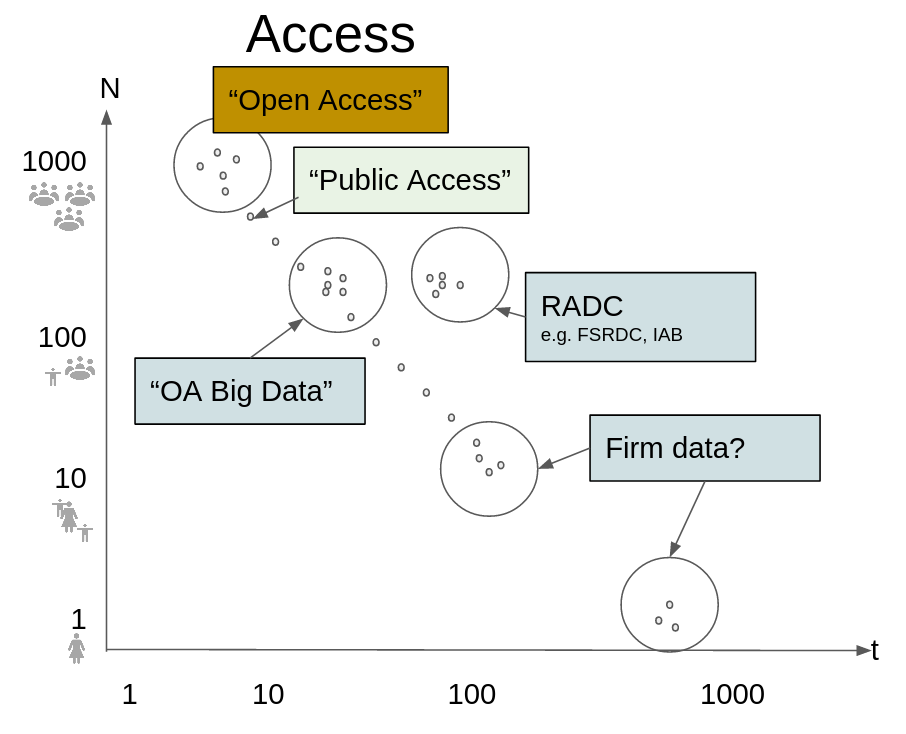
\includegraphics[width=0.8\textwidth]{figure1.png}
    \caption{Conceptual trade-off between number of individuals accessing data, and time required to do so. Figure first published in \citet{vilhuber_reproducibility_2023}.}
    \label{fig:nxt}
\end{figure}

\section{Data Access}
\label{sec:data_access}


\section{Access to Software}
\label{sec:software}

\section{Access to Resources}
\label{sec:other_resources}

In the template README suggested by several data editors in economics \parencite{templateREADMEv1.1}, we emphasize that a README should provide enough instructions for a reasonable person to re-implement the analysis described in the replication package. Here, authors need to take into account that cutting edge methods, including technology, may require more information and instruction than for standard methods. Authors likely do not need to describe how to run an analysis in Stata, given its ubiquitous use in economics, and the ease with which instructions can be found more generally, but they may need to provide detailed step-by-step information if the technology used is rare or bespoke. For instance, the emerging use of \acp{LLM} and \ac{AI} methods is far from the economic mainstream as of the writing of this article. Recent articles are still identifying ways economists scan actually use these tools, both for personal productivity \parencite{korinek_generative_2023} and as part of the technical toolkit \parencite{athey_machine_2019,dell_deep_2024}. Only one of the articles submitted to any of the AEA journals in 2024 used these techniques (to be named, not yet published).

The most recent modern toolkits are not the only resource constraints that might restrict broad access. While it might be argued that the use of proprietary software is restrictive, it is one of many resource constraints that may be binding for some researchers. Researchers in lower-ranked (and lower-funded) research institutions, including in \acp{LMIC}, may well not have the funds to purchase proprietary software, but access to computers may be equally constraining. The template README requests information on the type of computer that was used by the original researcher, to provide a benchmark to future re-users. Acquiring access to sufficient memory (\ac{RAM}), storage, and use over time of those resources can be expensive, even when renting such resources in cloud environments (which very few researchers appear to be doing). Traditionally, that access may be embedded within a single purchased computer, which may have (in 2024) around 32GB of RAM, 1-2 TB of storage, and have 4-12 compute cores available exclusively to the owner. More complex analyses may require access to compute clusters (using hundreds or thousands of compute cores), very large storage arrays (measured in the two- to three-digit TB range), and may require up to 1024 GB of RAM. Cutting edge analyses may require specialized chips, such as one or more \acp{GPU}, or even a cluster of \acp{GPU}. We have observed analyses that may run data cleaning or data acquisition processes for months at a time. 

The vast majority of articles published in economics journals usually require no more computing resources than a modern laptop provides, in all the dimensions enumerated in the previous paragraphy. In fact, a formal quantitative measurement of resource usage in economics articles is surprisingly hard to obtain, as most researchers are not very good at reporting the resources they have used to conduct their research. In part, this is because measuring such usage is non-trivial, but to a larger extent, I postulate that this is because most research institutions provide such resources to their researchers in a ``convenient way,'' and researchers conduct research within those constraints. More importantly, however, it suggests an important constraint on how ``open'' access can be for some if not all economics research.

\section{Open Infrastructure: Publications}
\label{sec:publications}

The challenges of openly accessible written scholarship are manifold, with the current focus on ``Plan S'', master publication agreements, and in the US, similar efforts under the moniker of the ``Nelson memo'' \parencite{brainard_white_2022,brainard_us_2024}. I note that the economics profession has a very long history of making much of the written knowledge available at very low cost via working papers \parencite{vilhuber_reproducibility_2020}, with the first working papers at the reputable NBER working paper series going back to 1973 \parencite{welch_education_1973}.

At the time of this writing, I have three editorial appointments. I am the Data Editor for the journals of the \acf{AEA}, the joint executive editor for the open access and multi-disciplinary \ac{JPC}, and I am a column editor for the open access \ac{HDSR}. I will use each of these to highlight a particular pattern in broadening access to publications, without any claim to generality. 

The \ac{AEA} is a not-for-profit organization, as are many other learned societies. It self-publishes eight journals, plus the proceedings of the annual conference, without relying on a commercial publishing house. Depending on the measurement, three of these publications are in the top ten journals in economics \citep{mogstad_statistical_2022-1}. Its publication costs account for about half of its overall operating expenses, and are only partially offset by directly attributable subscription and membership fees \citep{cherry_bekaert_llp_american_2024}. In fact, 6 of the top 10 journals in economics \citep{mogstad_statistical_2022-1} are published by societies (JEL, JEP, Econometrica, AER, Restud, JOLE), some of which have as sole or primary purpose the publication of the journal.\footnote{JOLE is a bit of an outlier, in that one becomes a member of the Society of Labor Economists by subscribing to the journal, rather than the other way around.} A further three journals are primarily associated with economics departments (QJE, JPE, RESTAT), which arguably may not be driven by pure profit. The sole outlier in the top ten is the \ac{JFE}, which is owned by Elsevier, a big commercial publisher. It should be noted that the \ac{EEA} severed its relationship with Elsevier in 2003 for its official journal, creating a journal that is fully owned by the association, adding to the list of society-owned journals in economics \citep{tirole_editorial_2003}. Access to these journals is generally still on a subscription basis (JEP is the exception, being free to read), but given the primarily not-for-profit organization of its owners, personal subscriptions (often via society membership) are quite low, compared to journals in many other sciences. For instance, as of 2024, a personal subscription to the Review of Economic Studies is \$156 or €141 per annum; a yearly membership to the \ac{AEA}, providing access to the seven subscription journals and the proceedings is \$25 for students and researchers in low-income countries, and \$150 at the highest personal income tier. As outlined earlier for the AEA, these subscription fees cover only a small fraction of the production costs. Nevertheless, even these (arguably low) costs do not satisfy ``Plan S'' or ``Nelson memo'' requirements, which require no access cost to the end consumer, and in the case of ``Plan S'', also require a liberal license allowing for re-use.\footnote{``The author(s) [...] grant(s) [...] a free, irrevocable, worldwide, right of access to, and a license to copy, use, distribute, transmit and display the work publicly and to make and distribute derivative works, [...] subject to proper attribution of authorship'' \citep{max-planck-gesellschaft_berlin_2023}. }

Interestingly in the context of the previous sections, all of the society-owned journals in the previous paragraph have appointed  data (reproducibility) editors.\footnote{Two additional societies, not previously mentioned, also employ data editors: the \ac{CEA} and the \ac{WEAI}. }

Since 2018, I have been the executive editor of the \ac{JPC}, an open access multi-disciplinary journal, having taken over the journal from Stephen Fienberg \citep{vilhuber_relaunching_2018}.\footnote{Fienberg, together with Cynthia Dwork and Alan Karr, founded the journal in 2009 \citep{abowd_first_2009}. Fienberg passed away in 2016 \citep{slavkovic_remembering_2018}.  In 2023, I recruited Rachel Cummings to jointly manage the journal.} As of 2024, the journal does not charge submission fees, and is free to read (what is called ``diamond open access.'' Articles default to a Creative Commons Attribution-NonCommercial-NoDerivatives (CC-BY-NC-ND) license, though authors are allowed to choose a more liberal license, for instance to comply with ``Plan S'' (which does not allow for the ``no-derivatives'' part). As executive editor, I have been responsible for all aspects of running the journal, not just finding referees for the articles that I am responsible for. The journal is made available through open-source software called Open Journal System, hosted by its creators at \href{https://pkp.sfu.ca/hosting-services/hosting/journals/}{Simon Fraser University's Public Knowledge Project}, preserved via industry-standard mechanisms (\href{https://clockss.org/about/how-clockss-works/}{CLOCKSS}, a non-profit) in case the journal ever needs to shut down, indexed in a variety of academic indexes, including via assignment of \acs{DOI}. Copy-editing is done through a mixture of professional copy-editors and volunteer work by editors and board members. All editors, including myself, are unpaid, and referees are, like in much of the publishing industry, unpaid volunteers. Yet I do pay bills, for each of the above components of a properly managed, indexed, and preserved academic journal --- and professional copy-editors and university staff do not work for free. I am thus quite aware of the absolute minimum cost of running a (small) journal. Over the years, funding has come from a variety of chaired professorships at Carnegie Mellon (Fienberg), Cornell (Abowd), and Harvard (Dwork). In order to make such funding more robust, a non-profit society was created to better and more robustly structure the funding situation \citep{abowd_launching_2024}. Time will tell if this will stabilize the funding situation, while maintaining the foundational commitment to open access. Others, in particular \href{https://sociologicalscience.com/}{Sociological Science}, have shown that it is feasible to sustainably publish high-quality research 


\section{Conclusion}

\printbibliography[title={References}]
\end{document}


\end{document}
